\documentclass{article}
\usepackage[left=1in, right=1in, top=1in, bottom=1in]{geometry}

\usepackage[utf8]{inputenc}
%\usepackage[T1]{fontenc}
\usepackage[croatian]{babel}

\usepackage{tikz}
\usepackage{float}

\title{Matemati\v{c}ki softver, 1. zada\'{c}a}

\begin{document}
\section{Popis tipova entiteta, veza i atributa}
Najprije slijede tipovi entiteta sa pripadnim atributima.
\begin{enumerate}
\item Tip entiteta KORISNIK sa atributima OIB (jedinstveni), IME, PREZIME, E-MAIL, HASH\_PASSWORD, REGISTRIRAN.
\item Tip entiteta RA\v{C}UN sa atributima ID (jedinstveni), TIP\_RA\v{C}UNA, VALUTA\_RA\v{C}UNA, STANJE\_RA\v{Č}UNA, DATUM\_IZRADE.
\item Tip entiteta TRANSAKCIJA sa atributima ID (jedinstveni), VALUTA, IZNOS, DATUM.
\item Tip entiteta PREDLO\v{Z}AK sa atributima ID (jedinstveni), VALUTA, IZNOS.
\item Tip entiteta PERIODI\v{C}NA\_TRANSAKCIJA sa atributima ID (jedinstveni), VALUTA, IZNOS, PERIOD, DATUM\_SLJEDE\'{C}E.
\item Tip entiteta \v{S}TEDNJA sa atributima ID (jedinstveni),  IZNOS\_\v{S}TEDNJE, KAMATNA\_STOPA.
\item Tip entiteta KREDIT sa atributima ID (jedinstveni), IZNOS\_KREDITA, KAMATNA\_STOPA, RATA\_PLA\'{C}ANJA.
\end{enumerate}
Sada slijede veze izme\dj u tipova entiteta.
\begin{enumerate}
\item VLASNIK\_RA\v{C}UNA, 1 : N veza izme\dj u KORISNIK i RA\v{C}UN. \v{C}lanstvo tipa entiteta RA\v{C}UN je obavezno.
\item \v{S}ALJE, 1 : N veza izme\dj u RA\v{C}UN i TRANSAKCIJA. \v{C}lanstvo tipa entiteta TRANSAKCIJA je obavezno.
\item PRIMA, 1 : N veza izme\dj u RA\v{C}UN i TRANSAKCIJA. \v{C}lanstvo tipa entiteta TRANSAKCIJA je obavezno.
\item PREDLO\v{Z}AK\_\v{S}ALJE, 1 : N veza izme\dj u RA\v{C}UN i PREDLO\v{Z}AK. \v{C}lanstvo tipa entiteta PREDLO\v{Z}AK je obavezno.
\item PREDLO\v{Z}AK\_PRIMA, 1 : N veza izme\dj u RA\v{C}UN i PREDLO\v{Z}AK. \v{C}lanstvo tipa entiteta PREDLO\v{Z}AK je obavezno.
\item PERIODI\v{C}NO\_\v{S}ALJE, 1 : N veza izme\dj u RA\v{C}UN i PERIODI\v{C}NA\_TRANSAKCIJA. \v{C}lanstvo tipa entiteta PERIODI\v{C}NA\_TRANSAKCIJA je obavezno.
\item PERIODI\v{C}NO\_PRIMA, 1 : N veza izme\dj u RA\v{C}UN i PERIODI\v{C}NA\_TRANSAKCIJA. \v{C}lanstvo tipa entiteta PERIODI\v{C}NA\_TRANSAKCIJA je obavezno.
\item VLASNIK\_\v{S}TEDNJE, 1 : N veza izme\dj u KORISNIK i \v{S}TEDNJA. \v{C}lanstvo tipa entiteta \v{S}TEDNJA je obavezno.
\item IMATELJ\_KREDITA, 1 : N veza izme\dj u KORISNIK i KREDIT. \v{C}lanstvo tipa entiteta KREDIT je obavezno.
\end{enumerate}
Dijagram ER sheme je na sljede\'{c}oj stranici. Nije prikazana cijela baza, ali ostalo se lako uvede iz ve\'{c} postoje\'{c}eg.

\newpage

\begin{figure}[H]
\centering
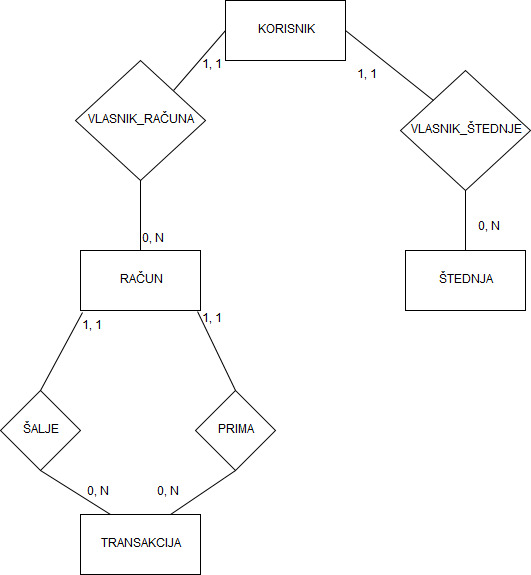
\includegraphics[width=1\textwidth]{er.jpg}
\end{figure}

\newpage

\section{Relacijska shema baze}
Sada pretvaramo prije opisane tipove entiteta i veza u relacije. \\

KORISNIK(\underline{OIB}, IME, PREZIME, E-MAIL, HASH\_PASSWORD, REGISTRIRAN)\\
RA\v{C}UN(\underline{ID}, OIB, TIP\_RA\v{C}UNA, VALUTA\_RA\v{C}UNA, STANJE\_RA\v{C}UNA, DATUM\_IZRADE)
TRANSAKCIJA(\underline{ID}, RA\v{C}UN\_PO\v{S}ILJATELJ, RA\v{C}UN\_PRIMATELJ, VALUTA, IZNOS, DATUM)\\
PREDLO\v{Z}AK(\underline{ID}, RA\v{C}UN\_PO\v{S}ILJATELJ, RA\v{C}UN\_PRIMATELJ, VALUTA, IZNOS)\\
PERIODI\v{C}NA\_TRANSAKCIJA(\underline{ID}, RA\v{C}UN\_PO\v{S}ILJATELJ, RA\v{C}UN\_PRIMATELJ, VALUTA, IZNOS, PERIOD, DATUM\_SLJEDE\'{C}E)\\
\v{S}TEDNJA(\underline{ID}, OIB, IZNOS\_\v{S}TEDNJE, KAMATNA\_STOPA, VALUTA) \\
KREDIT(\underline{ID}, OIB, IZNOS\_KREDITA, KAMATNA\_STOPA, RATA\_PLA\'{C}ANJA, VALUTA) \\

S obzirom da su sve veze 1 : N gdje je jedan entitet u obaveznom \v{c}lanstvu, lako smo ih uvrstili kao atribute relacija (npr. u RA\v{C}UN smo dodali OIB koji govori tko mu je vlasnik). 

\newpage

\section{Rje\v{c}nik podataka}
\begin{center}
\begin{tabular}{|c|c|c|}
\hline
\textbf{IME ATRIBUTA} & \textbf{TIP} & \textbf{KRATKI OPIS} \\
\hline
OIB & Niz od to\v{c}no 11 znamenki & Jednozna\v{c}no odre\dj uje osobu. \\
\hline
IME & Niz znakova & Ime korisnika \\
\hline
PREZIME & Niz znakova & Prezime korisnika \\
\hline
E-MAIL & Niz znakova & E-mail korisnika \\
\hline
HASH\_PASSWORD & Niz znakova & (Hashirana) lozinka korisnika \\
\hline
REGISTRIRAN & 0 ili 1 & Sugerira je li korisnik dovr\v{s}io registraciju \\
\hline
ID & Broj & Odre\dj uje jedinstvenost entiteta unutar nekog tipa\\
\hline
TIP\_RA\v{C}UNA & Niz znakova & Npr. teku\'{c}i ra\v{c}un, devizni ra\v{c}un\ldots \\
\hline
VALUTA & Niz od 3 znaka & Valuta u kojoj se vr\v{s}i (ili \'{c}e se vr\v{s}iti) transakcija \\
\hline
STANJE\_RA\v{C}UNA & Decimalni broj s dvije decimale & Koliko korisnik ima sredstava na ra\v{c}unu \\
\hline
DATUM & Datum & Jasno je iz konteksta, tj. unutar kojeg tipa se nalazi \\
\hline
RA\v{C}UN\_PO\v{S}ILJATELJ & Broj & ID ra\v{c}una koji \v{s}alje sredstva putem transakcije. \\
\hline
RA\v{C}UN\_PRIMATELJ & Broj & ID ra\v{c}una koji prima sredstva putem transakcije. \\
\hline
IZNOS & Decimalni broj s dvije decimale & Koliko se sredstva poslalo (ili \'{c}e se poslati) \\
\hline
PERIOD & Broj & Period pla\'{c}anja u mjesecima \\
\hline
KAMATNA\_STOPA & Decimalni broj s dvije decimale & Kamatna stopa na kredit ili na \v{s}tednju \\
\hline
IZNOS\_\v{S}TEDNJE & Decimalni broj s dvije decimale & Trenutni iznos sredstava namijenjenih \v{s}tednji \\
\hline
IZNOS\_KREDITA & Decimalni broj s dvije decimale & Koliko jo\v{s} korisnik mora pla\'{c}ati kredit \\
\hline
RATA\_PLA\'{C}ANJA & Decimalni broj s dvije decimale & Koliko korisnik otpla\'{c}uje kredita u jednoj rati. \\
\hline
\end{tabular}
\end{center}
\newpage
\section{Fizi\v{c}ka shema baze}
Ovdje nije dana, vidjeti .php file koji se koristio za izradu baze.
\end{document}